\documentclass[11pt, oneside]{article}   	% use "amsart" instead of "article" for AMSLaTeX format


%\usepackage{draftwatermark}
% \SetWatermarkText{Confidential}
% \SetWatermarkScale{5}
% \SetWatermarkLightness {0.85} 
% \SetWatermarkColor[rgb]{0.7,0,0}


\usepackage{geometry}                		% See geometry.pdf to learn the layout options. There are lots.
\geometry{letterpaper}                   		% ... or a4paper or a5paper or ... 
%\geometry{landscape}                		% Activate for for rotated page geometry
%\usepackage[parfill]{parskip}    		% Activate to begin paragraphs with an empty line rather than an indent
\usepackage{graphicx}				% Use pdf, png, jpg, or eps� with pdflatex; use eps in DVI mode
								% TeX will automatically convert eps --> pdf in pdflatex		
\usepackage{amssymb}
\usepackage{mathrsfs}
\usepackage{hyperref}
\usepackage{url}
\usepackage{authblk}
\usepackage{amsmath}
\usepackage{mathtools}
\usepackage{graphicx}
\usepackage{fixltx2e}
\usepackage{hyperref}
\usepackage{alltt}
\usepackage{color}

\newcommand{\argmax}{\operatornamewithlimits{argmax}}
\newcommand{\argmin}{\operatornamewithlimits{argmin}}



\title{Some notes on Policy Gradients for Reinforcement Learning}
\author{David Meyer \\ dmm@\{1-4-5.net,uoregon.edu,...\}}

\date{Last update: \today}							% Activate to display a given date or no date


\begin{document}
\maketitle

\section{Introduction} 
\label{sec:intro}
Policy gradients for Reinforcement Learning (RL) are really beautiful in form and function. In these notes I'll try to point out a few of these amazing features\footnote{Here we follow the notation used in \cite{SuttonBook}.}.

\bigskip
\noindent
Here we consider methods that learn a parameterized policy that can select actions without consulting a value function. A value function may still be used to learn the policy weights, but that is not required for action selection. The notation $\theta \in \mathbb{R}^n$ is typically used for the primary learned weight vector, and $\pi(a \mid s, \theta) = Pr(A_t = a \mid s_t = s, \theta_t = \theta)$  is the probability that action $a$ is taken at time $t$ given that the agent is in state $s$ at time $t$ with weight vector $\theta$. If a method uses a learned value function as well, then the value function's weight vector is denoted $w$ to distinguish it from $\theta$, such as in $\hat{v}(s,w)$.

\bigskip
\noindent
We wish to consider methods for learning the policy weights $\theta$ based on the gradient of some performance measure $\eta(\theta)$) with respect to the policy weights. These methods seek to maximize performance, so their updates approximate gradient ascent in $\eta$. As is typical for gradient descent/ascent, 
\begin{flalign}
\boldsymbol{\theta}_{t+1} \coloneqq \boldsymbol{\theta}_t + \alpha \widehat{\nabla \eta(\boldsymbol{\theta}_t)}
\end{flalign}

\noindent
where, as is typical with gradient ascent/decent methods, $\widehat{\nabla \eta(\boldsymbol{\theta}_t)}$ is a stochastic estimate whose expectation approximates the gradient of the performance measure $\eta$ with respect to its argument $\theta_t$. As we will see, $\widehat{\nabla \eta(\boldsymbol{\theta}_t)}$ will turn out to be something like $\nabla_{\theta} \mathbb{E}_{\tau}[R(\tau)]$, where $\tau$ is a \emph{trajectory} and $R(\tau)$ is the return for path $\tau$ (see Section \ref{sec:scorefunction}).

\section{Score Function/Likelihood Ratio Estimators}
\label{sec:scorefunction}

First notices that Likelihood Ratio methods only change the probabilities of experienced paths, and further, these methods do not try to change the actions taken in a given path. 
That said, recall that our problem here is to solve the following:

\begin{flalign}
 \max_\theta \mathbb{E}[\sum\limits_{t = 0}^{H} R(s_t) \mid \pi_\theta]
\end{flalign}

\noindent 
where $\pi_{\theta}(u \mid s)$ is the probability of action $u$ in state $s$.
Now, because ultimately we'll want to compute the gradient $\nabla_{\theta} \mathbb{E}[R \mid \pi_\theta]$,  we need to prove one identity, namely (imagine that $f(x) = R$)

\begin{flalign}
\nabla_{\theta} \mathbb{E}_{x \sim p(x \mid \theta)} [f(x)] =  \mathbb{E}_{x} [f(x) \nabla_{\theta} \log p(x  \mid  \theta)]
\label{eqn:E}
\end{flalign}

\bigskip
\noindent
So the proof of this is amazingly simple given the log derivative trick\footnote{\url{http://blog.shakirm.com/2015/11/machine-learning-trick-of-the-day-5-log-derivative-trick}}. First, consider a function $f(x)$ for which we wish to find 
$\nabla_{\theta} \mathbb{E}_{x \sim p(x \mid \theta)} [f(x)]$. Then
\begin{flalign}
\nabla_{\theta} \mathbb{E}_{x \sim p(x \mid \theta)} [f(x)] 
&= \nabla_{\theta} \int_x p(x \mid \theta) f(x) dx  \; \quad \qquad \qquad \mathbin{\#} \text{definition} \\
&= \int_x \nabla_{\theta} p(x \mid \theta) f(x) dx  \; \quad \qquad \qquad \mathrel{\#} \text{Lebesgue Integral} \\
&= \int_x p(x \mid \theta) \frac{\nabla_{\theta} p(x \mid \theta)} {p(x \mid \theta)} f(x) dx   \qquad \mathrel{\#} \text{multiply by }  \frac{p(x \mid \theta)}{p(x \mid \theta)} \\
&= \int_x p(x \mid \theta)  \nabla_{\theta} \log{p(x \mid \theta)} f(x)  \qquad \mathrel{\#} \text{log-derivative trick} \\
&= \mathbb{E}_{x \sim p(x \mid \theta)} [f(x) \nabla_{\theta} \log{p(x \mid \theta)}] \qquad \mathrel{\#} \text{defn expectation} 
\end{flalign}

\bigskip
\noindent
Define $\hat{g}_i = f(x_i)  \nabla_\theta \log p(x_i  \mid  \theta)$.  An empirical estimate the gradient for $m$ samples is
\begin{flalign}
\nabla_{\theta} \mathbb{E}_{x \sim p(x \mid \theta)} [f(x)] 
= g \approx \frac{1}{m} \sum\limits_{i = 1}^{m} \hat{g}_i 
= \frac{1}{m} \sum\limits_{i = 1}^{m} f(x_i)  \nabla_\theta \log p(x_i  \mid  \theta)
\end{flalign}

\bigskip
\noindent
Aside:  The "log derivative trick", which is also called the "likelihood ratio trick" since $\frac{\nabla_{\theta} p(x \mid \theta)}{p(x \mid \theta)}$ is called the "likelihood ratio" and
$\frac{\nabla_{\theta} p(x \mid \theta)}{p(x \mid \theta)} = \nabla_{\theta} \log  p(x \mid \theta)$,  
is sometimes framed up like this: The gradient of something divided by something is the gradient of  log something. Also frequently
pronounced "grad something divided by something is grad log something".



\bigskip
\noindent
So $\nabla_{\theta} E_{x \sim p(x \mid \theta)} [f(x)] =  E_{x \sim p(x \mid \theta)} [f(x) \nabla_{\theta} \log{p(x \mid \theta)}]$. 
This gives us an unbiased gradient estimator; to compute the gradient estimate, just sample $x_i \sim p(x  \mid \theta)$ and then compute the gradient estimate
$\hat{g}_i = f(x_i)  \nabla_\theta \log p(x_i  \mid  \theta)$. Now, let the trajectory (sometimes path)  $\tau$ be the state-action sequence  $(s_0,a_0, r_0,s_1,a_1,r_1,\cdots, a_{T-1}, a_{T-1},r_{T-1})$ and suppose $f(x) = R(\tau)$, the total return for \emph{path} $\tau$. Then

\bigskip

\begin{flalign}
\nabla_{\theta} \mathbb{E}_{\tau}[R(\tau)] &= E_{\tau} [\nabla_{\theta} \log{p(\tau \mid \theta)} R(\tau) ]
\label{eqn:gradient}
\end{flalign}

\bigskip
\noindent
so that all we really need to do is see that we can compute $p(\tau \mid \theta)$:

\begin{flalign}
p(\tau \mid \theta) &= \mu_0(s_0) \prod\limits_{t = 0}^{T - 1} \underbrace{\pi(a_t \mid s_t,\theta)}_{\text{policy}} \underbrace{P(s_{t+1},r_t) \mid s_t,a_t)}_{\text{dynamics}} 
\qquad \qquad \mathbin{\#} \text{definition }\\
\log p(\tau \mid \theta) &= \log{\mu_0(s_0)} + \sum\limits_{t = 0}^{T-1} \log{\pi(a_t \mid s_t,\theta)} + \log{P(s_{t+1},r_t) \mid s_t,a_t)} \\
\nabla_{\theta} \log p(\tau \mid \theta) &= \nabla_{\theta} \sum\limits_{t = 0}^{T-1}\log{\pi(a_t \mid s_t,\theta)} \\
&= \sum\limits_{t = 0}^{T-1} \nabla_{\theta}  \log{\pi(a_t \mid s_t,\theta)} 
\end{flalign}

\bigskip
\noindent
So $\nabla_{\theta} \mathbb{E}_{\tau} [R] = \mathbb{E}_{\tau} [R(\tau) \nabla_{\theta} \sum\limits_{t = 0}^{T-1} \log{\pi(a_t \mid s_t,\theta)}]$, which gives a direct way of computing a gradient we can use with standard Stochastic Gradient Ascent (or Descent), where the parameter update rule would be something like $\theta \coloneqq \theta + \alpha \nabla_{\theta} \mathbb{E}_{\tau}[R(\tau)]$. Essentially move $\theta$ in the direction of better expected return. Note also that the model dynamics, $P(s_{t+1},r_t) \mid s_t,a_t)$, conveniently drops out of the gradient (good thing given that we're trying to learn model-free control).

\section{Derivation of the Gradient via Importance Sampling}

It turns out that almost all on-policy control methods utilize importance sampling, which is a general technique for estimating expected values under one distribution given samples from another\cite{SuttonBook}. The basic approach to applying importance sampling to on-policy learning is by weighting returns according to the relative probability of their trajectories occurring under the target and behavior policies; this is called the importance-sampling ratio. Now given a starting state $S_t$, the probability of the subsequent state-action trajectory 
$\tau = A_t,S_{t+1},A_{t+1} \cdots,S_T$ occurring under any policy $\pi$  is
\begin{flalign} 
p_t(\tau) &= \prod\limits_{k=t}^{T-1} \pi(A_k \mid S_k) p(S_{k+1} \mid S_k,A_k)
\end{flalign}
\noindent
where $p$ is the state-transition probability function. The relative probability of the trajectory under the target and behavior policies (the importance-sampling ratio) is then
\begin{flalign} 
\rho_t^T =\frac{ \prod\limits_{k=t}^{T-1} \pi(A_k \mid S_k) p(S_{k+1} \mid S_k,A_k)}{\prod\limits_{k=t}^{T-1} u(A_k \mid S_k) p(S_{k+1} \mid S_k,A_k)}
&= \frac{ \prod\limits_{k=t}^{T-1} \pi(A_k \mid S_k)}{\prod\limits_{k=t}^{T-1} u(A_k \mid S_k)}
\end{flalign}

\begin{figure}
\center{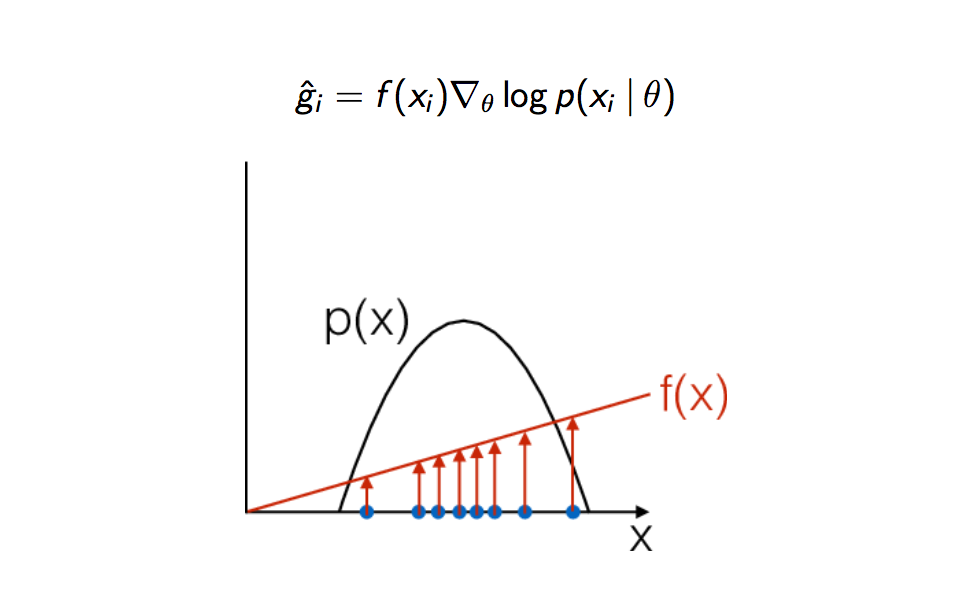
\includegraphics[scale=0.6] {images/score_function_gradient_estimator_1.png}}
\caption{Score/likelihood Gradient Estimator Intuition 1. Image courtesy John Schulman \url{https://learning.mpi-sws.org/mlss2016/slides/2016-MLSS-RL.pdf}}
\label{fig:slge1}
\end{figure}


\noindent
One of the many interesting things here is that it turns out that $\rho_t^T$ doesn't depend on the MDP's transition probability function (which is what we want since we want to solve the model-free problem). In the following example, consider $\rho_t^T = \frac{p(x  \mid  \theta)}{p(x  \mid  \theta_{\textrm old})}$.

\begin{flalign} 
\mathbb{E}_{x \sim \theta} \big[ f(x) \big ] & = \mathbb{E}_{x \sim \theta_{\textrm old}} \Bigg [\frac{p(x  \mid  \theta)}{p(x  \mid  \theta_{\textrm old})} f(x) \Bigg] \\
\nabla_{\theta} \mathbb{E}_{x \sim \theta} \big [f(x) \big ] 
&= \mathbb{E}_{x \sim \theta_{\textrm old}} \Bigg [\frac{\nabla_{\theta} p(x  \mid  \theta)}{p(x  \mid  \theta_{\textrm old})} f(x) \Bigg] \\
\nabla_{\theta} \mathbb{E}_{x \sim \theta} \big [ f(x) \big ] \bigr |_{\theta = \theta_{\textrm old}}
 &= \mathbb{E}_{x \sim \theta_{\textrm old}} \Bigg [\frac{\nabla_{\theta} p(x  \mid  \theta) \bigr |_{\theta = \theta_{\textrm old}}}{p(x  \mid  \theta_{\textrm old})} f(x) \Bigg] \\
 &= \mathbb{E}_{x \sim \theta_{\textrm old}} \Bigg [\nabla_{\theta} \log p(x \mid \theta) \bigr |_{\theta = \theta_{\textrm old}} f(x) \Bigg] 
\end{flalign}


\begin{figure}
\center{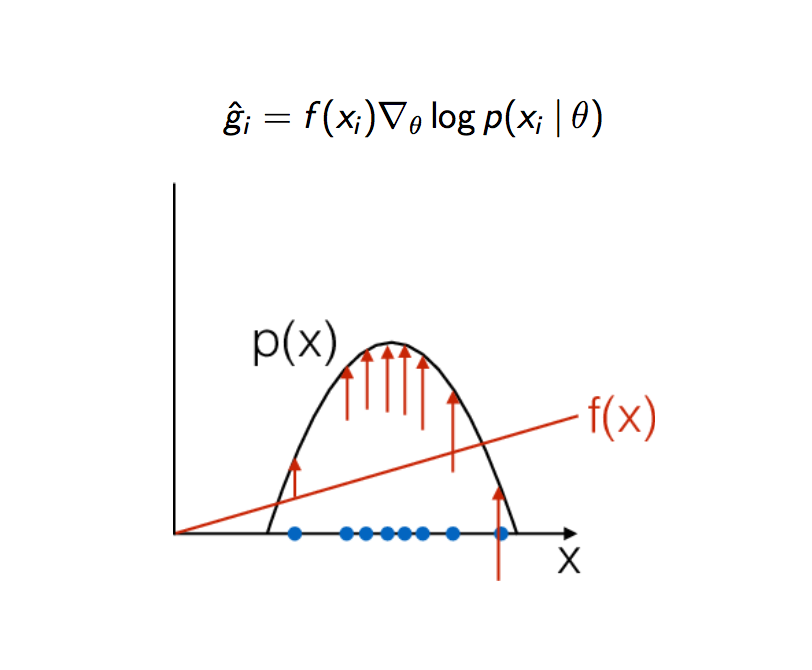
\includegraphics[scale=0.6] {images/score_function_gradient_estimator_2.png}}
\caption{Score/likelihood Gradient Estimator Intuition 2. Image courtesy John Schulman \url{https://learning.mpi-sws.org/mlss2016/slides/2016-MLSS-RL.pdf}}
\label{fig:slge2}
\end{figure}


\section{A Bit of Intuition}

What we've learned so far is that we can compute the an estimate of the gradient for sample $i$ is $\hat{g}_i = f(x_i)\nabla_{\theta} \log p(x_i \mid \theta)$. Now, suppose $f(x)$ somehow measures how good the sample $x$ is. Then we can conclude a few things about $\hat{g}_i$:
\begin{itemize}
\item Moving in the direction $\hat{g}_i$ pushes up the log probability ("logprob")  of the sample in proportion to how good it is (i.e., $f(x_i)$), remembering that the SGD update rule is something like $\theta \coloneqq  \theta + \alpha \nabla_{\theta} \mathbb{E}_{\tau}[R(\tau)]$. This pushing up is depicted in Figures \ref{fig:slge1} and \ref{fig:slge2}.
\item Note that this is true even if $f (x )$ is discontinuous, and unknown, or the sample space (containing $x$) is a discrete set!
\item More generally, Maximum Likelihood Estimation (MLE) consists of taking several samples from the Data Generating Distribution (DGD) to form a training set, then pushing up on the probability the model assigns to those points, thus maximizing the likelihood of the training data. Figure \ref{fig:mle} shows how different data points push up on different parts of
the density function for a Gaussian model applied to 1-D data. The fact that the density function must sum to one means that we cannot simply assign infinite likelihood to all points; as one point pushes up in one place it inevitably pulls down in other places. The resulting density function balances out the upward forces from all the data points in different locations.
\end{itemize}
Basically, the gradient tries to Increase probability of paths with	positive return R and decrease the probability of paths with negative return.
\begin{figure}
\center{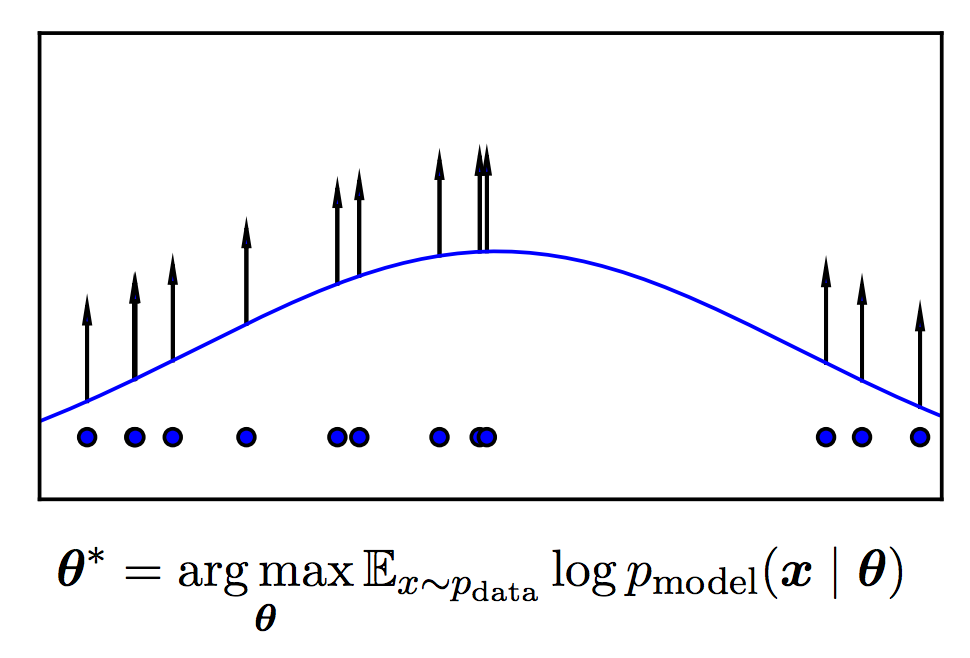
\includegraphics[scale=0.6] {images/mle.png}}
\caption{Maximum Likelihood Estimation. Image courtesy Ian Goodfellow \cite{Goodfellow:2017aa}.}
\label{fig:mle}
\end{figure}


\subsection{Reorganizing Equation \ref{eqn:gradient}}

Equation \ref{eqn:gradient} can be rewritten as follows:

\begin{flalign}
\nabla_{\theta} \mathbb{E}_{\tau}[R(\tau)] &= E_{\tau} [\nabla_{\theta} \log{p(\tau \mid \theta)} R(\tau) ] \\
&= \mathbb{E} \Bigg [ \Bigg (\sum\limits_{t = 0}^{T - 1} r_t \Bigg) \Bigg(\sum\limits_{t = 0}^{T - 1}  \nabla_{\theta} \log{\pi(a_t \mid s_t,\theta)}\Bigg ) \Bigg ]
\end{flalign}

\bigskip
\noindent
But notice that we can limit the trajectory to $t$ steps and derive gradient estimator for one reward term $r_{t^\prime}$. In particular

\begin{flalign}
\nabla_{\theta}\mathbb{E}\big[r_{t^\prime}\big] &= \mathbb{E} \Bigg [ r_{t^\prime} \sum\limits_{t = 0}^{t} \nabla_{\theta} \log{\pi(a_t \mid s_t,\theta)} \Bigg ]
\end{flalign}

\bigskip
\noindent
Now, we can sum over $t$ to get

\begin{flalign}
\nabla_{\theta}\mathbb{E}\big[R\big] &= \mathbb{E} \Bigg [\sum\limits_{t^\prime = 0}^{T - 1} r_{t^\prime} \sum\limits_{t = 0}^{T-1}\nabla_{\theta} \log{\pi(a_t \mid s_t,\theta)} \Bigg ] \\
&= \mathbb{E}\Bigg [\sum\limits_{t = 0}^{T - 1} \nabla_{\theta} \log{\pi(a_t \mid s_t,\theta)} \sum\limits_{t^{\prime} = t}^{T-1} r_{t^\prime} \Bigg]
\end{flalign}

\section{Adding a Baseline: Deriving an Unbiased Estimator}
Here's the problem:  suppose that $f(x) \ge 0 \; \forall x$. Then for every $x_i$, the gradient estimator $\hat{g}_i$ tries to push up up its density (recall that $\boldsymbol{\theta}_{t+1} \coloneqq \boldsymbol{\theta}_t + \alpha \widehat{\nabla \eta(\boldsymbol{\theta}_t)}$). Better would be to have a (new) unbiased estimator that avoids this problem; this estimator would only push up the density for better-than-average $x_i$. What would this look like?

\begin{flalign}
\nabla_{\theta}\mathbb{E}_{x} \big[f(x)\big] &= \nabla_{\theta}\mathbb{E}_{x} \big[ (f(x) - b) \big] \\
&= \mathbb{E}_x \big [ \nabla_{\theta} \log p(x \mid \theta) (f(x) - b) \big ]
\end{flalign}

\bigskip
\noindent
Note that a near optimal choice for $b$ is always $\mathbb{E}\big[f(x)\big]$; however $\mathbb{E}\big[f(x)\big]$ must itself be estimated.

\bigskip
\noindent
To derive our estimate with baseline, recall that 

\begin{flalign}
\nabla_{\theta}\mathbb{E}_{\tau}\big[R\big] 
&= \Bigg [\sum\limits_{t^\prime = 0}^{T - 1} r_{t^\prime} \sum\limits_{t = t^{\prime}}^{t^\prime}\nabla_{\theta} \log{\pi(a_t \mid s_t,\theta)} \Bigg ]  \\
&= \mathbb{E}_{\tau} \Bigg [ \sum\limits_{t=0}^{T-1}  \log{\pi(a_t \mid s_t,\theta)} \Bigg ( \sum\limits_{t^{\prime} = t}^{T-1} r_{t^\prime} - b(s_t) \Bigg) \Bigg ]
\end{flalign}

\bigskip
\noindent
for any "baseline" function $b: \mathcal{S} \rightarrow \mathbb{R}$. See Schulman, J. , et al. \cite{Schulman:2015aa} for details of the proof.

\newpage
\bibliographystyle{ieeetr}
\bibliography{/Users/dmm/papers/bib/ml}



\end{document} 
